\documentclass{ximera}

%\usepackage{todonotes}

\newcommand{\todo}{}

\usepackage{esint} % for \oiint
\ifxake%%https://math.meta.stackexchange.com/questions/9973/how-do-you-render-a-closed-surface-double-integral
\renewcommand{\oiint}{{\large\bigcirc}\kern-1.56em\iint}
\fi


\graphicspath{
  {./}
  {ximeraTutorial/}
  {basicPhilosophy/}
  {functionsOfSeveralVariables/}
  {normalVectors/}
  {lagrangeMultipliers/}
  {vectorFields/}
  {greensTheorem/}
  {shapeOfThingsToCome/}
  {dotProducts/}
  {partialDerivativesAndTheGradientVector/}
  {../productAndQuotientRules/exercises/}
  {../normalVectors/exercisesParametricPlots/}
  {../continuityOfFunctionsOfSeveralVariables/exercises/}
  {../partialDerivativesAndTheGradientVector/exercises/}
  {../directionalDerivativeAndChainRule/exercises/}
  {../commonCoordinates/exercisesCylindricalCoordinates/}
  {../commonCoordinates/exercisesSphericalCoordinates/}
  {../greensTheorem/exercisesCurlAndLineIntegrals/}
  {../greensTheorem/exercisesDivergenceAndLineIntegrals/}
  {../shapeOfThingsToCome/exercisesDivergenceTheorem/}
  {../greensTheorem/}
  {../shapeOfThingsToCome/}
  {../separableDifferentialEquations/exercises/}
  {vectorFields/}
}

\newcommand{\mooculus}{\textsf{\textbf{MOOC}\textnormal{\textsf{ULUS}}}}

\usepackage{tkz-euclide}
\usepackage{tikz}
\usepackage{tikz-cd}
\usetikzlibrary{arrows}
\tikzset{>=stealth,commutative diagrams/.cd,
  arrow style=tikz,diagrams={>=stealth}} %% cool arrow head
\tikzset{shorten <>/.style={ shorten >=#1, shorten <=#1 } } %% allows shorter vectors

\usetikzlibrary{backgrounds} %% for boxes around graphs
\usetikzlibrary{shapes,positioning}  %% Clouds and stars
\usetikzlibrary{matrix} %% for matrix
\usepgfplotslibrary{polar} %% for polar plots
\usepgfplotslibrary{fillbetween} %% to shade area between curves in TikZ
%\usetkzobj{all}
\usepackage[makeroom]{cancel} %% for strike outs
%\usepackage{mathtools} %% for pretty underbrace % Breaks Ximera
%\usepackage{multicol}
\usepackage{pgffor} %% required for integral for loops



%% http://tex.stackexchange.com/questions/66490/drawing-a-tikz-arc-specifying-the-center
%% Draws beach ball
\tikzset{pics/carc/.style args={#1:#2:#3}{code={\draw[pic actions] (#1:#3) arc(#1:#2:#3);}}}



\usepackage{array}
\setlength{\extrarowheight}{+.1cm}
\newdimen\digitwidth
\settowidth\digitwidth{9}
\def\divrule#1#2{
\noalign{\moveright#1\digitwidth
\vbox{\hrule width#2\digitwidth}}}




% \newcommand{\RR}{\mathbb R}
% \newcommand{\R}{\mathbb R}
% \newcommand{\N}{\mathbb N}
% \newcommand{\Z}{\mathbb Z}

\newcommand{\sagemath}{\textsf{SageMath}}


%\renewcommand{\d}{\,d\!}
%\renewcommand{\d}{\mathop{}\!d}
%\newcommand{\dd}[2][]{\frac{\d #1}{\d #2}}
%\newcommand{\pp}[2][]{\frac{\partial #1}{\partial #2}}
% \renewcommand{\l}{\ell}
%\newcommand{\ddx}{\frac{d}{\d x}}

% \newcommand{\zeroOverZero}{\ensuremath{\boldsymbol{\tfrac{0}{0}}}}
%\newcommand{\inftyOverInfty}{\ensuremath{\boldsymbol{\tfrac{\infty}{\infty}}}}
%\newcommand{\zeroOverInfty}{\ensuremath{\boldsymbol{\tfrac{0}{\infty}}}}
%\newcommand{\zeroTimesInfty}{\ensuremath{\small\boldsymbol{0\cdot \infty}}}
%\newcommand{\inftyMinusInfty}{\ensuremath{\small\boldsymbol{\infty - \infty}}}
%\newcommand{\oneToInfty}{\ensuremath{\boldsymbol{1^\infty}}}
%\newcommand{\zeroToZero}{\ensuremath{\boldsymbol{0^0}}}
%\newcommand{\inftyToZero}{\ensuremath{\boldsymbol{\infty^0}}}



% \newcommand{\numOverZero}{\ensuremath{\boldsymbol{\tfrac{\#}{0}}}}
% \newcommand{\dfn}{\textbf}
% \newcommand{\unit}{\,\mathrm}
% \newcommand{\unit}{\mathop{}\!\mathrm}
% \newcommand{\eval}[1]{\bigg[ #1 \bigg]}
% \newcommand{\seq}[1]{\left( #1 \right)}
% \renewcommand{\epsilon}{\varepsilon}
% \renewcommand{\phi}{\varphi}


% \renewcommand{\iff}{\Leftrightarrow}

% \DeclareMathOperator{\arccot}{arccot}
% \DeclareMathOperator{\arcsec}{arcsec}
% \DeclareMathOperator{\arccsc}{arccsc}
% \DeclareMathOperator{\si}{Si}
% \DeclareMathOperator{\scal}{scal}
% \DeclareMathOperator{\sign}{sign}


%% \newcommand{\tightoverset}[2]{% for arrow vec
%%   \mathop{#2}\limits^{\vbox to -.5ex{\kern-0.75ex\hbox{$#1$}\vss}}}
% \newcommand{\arrowvec}[1]{{\overset{\rightharpoonup}{#1}}}
% \renewcommand{\vec}[1]{\arrowvec{\mathbf{#1}}}
% \renewcommand{\vec}[1]{{\overset{\boldsymbol{\rightharpoonup}}{\mathbf{#1}}}}

% \newcommand{\point}[1]{\left(#1\right)} %this allows \vector{ to be changed to \vector{ with a quick find and replace
% \newcommand{\pt}[1]{\mathbf{#1}} %this allows \vec{ to be changed to \vec{ with a quick find and replace
% \newcommand{\Lim}[2]{\lim_{\point{#1} \to \point{#2}}} %Bart, I changed this to point since I want to use it.  It runs through both of the exercise and exerciseE files in limits section, which is why it was in each document to start with.

% \DeclareMathOperator{\proj}{\mathbf{proj}}
% \newcommand{\veci}{{\boldsymbol{\hat{\imath}}}}
% \newcommand{\vecj}{{\boldsymbol{\hat{\jmath}}}}
% \newcommand{\veck}{{\boldsymbol{\hat{k}}}}
% \newcommand{\vecl}{\vec{\boldsymbol{\l}}}
% \newcommand{\uvec}[1]{\mathbf{\hat{#1}}}
% \newcommand{\utan}{\mathbf{\hat{t}}}
% \newcommand{\unormal}{\mathbf{\hat{n}}}
% \newcommand{\ubinormal}{\mathbf{\hat{b}}}

% \newcommand{\dotp}{\bullet}
% \newcommand{\cross}{\boldsymbol\times}
% \newcommand{\grad}{\boldsymbol\nabla}
% \newcommand{\divergence}{\grad\dotp}
% \newcommand{\curl}{\grad\cross}
%\DeclareMathOperator{\divergence}{divergence}
%\DeclareMathOperator{\curl}[1]{\grad\cross #1}
% \newcommand{\lto}{\mathop{\longrightarrow\,}\limits}

% \renewcommand{\bar}{\overline}

\colorlet{textColor}{black}
\colorlet{background}{white}
\colorlet{penColor}{blue!50!black} % Color of a curve in a plot
\colorlet{penColor2}{red!50!black}% Color of a curve in a plot
\colorlet{penColor3}{red!50!blue} % Color of a curve in a plot
\colorlet{penColor4}{green!50!black} % Color of a curve in a plot
\colorlet{penColor5}{orange!80!black} % Color of a curve in a plot
\colorlet{penColor6}{yellow!70!black} % Color of a curve in a plot
\colorlet{fill1}{penColor!20} % Color of fill in a plot
\colorlet{fill2}{penColor2!20} % Color of fill in a plot
\colorlet{fillp}{fill1} % Color of positive area
\colorlet{filln}{penColor2!20} % Color of negative area
\colorlet{fill3}{penColor3!20} % Fill
\colorlet{fill4}{penColor4!20} % Fill
\colorlet{fill5}{penColor5!20} % Fill
\colorlet{gridColor}{gray!50} % Color of grid in a plot

\newcommand{\surfaceColor}{violet}
\newcommand{\surfaceColorTwo}{redyellow}
\newcommand{\sliceColor}{greenyellow}




\pgfmathdeclarefunction{gauss}{2}{% gives gaussian
  \pgfmathparse{1/(#2*sqrt(2*pi))*exp(-((x-#1)^2)/(2*#2^2))}%
}


%%%%%%%%%%%%%
%% Vectors
%%%%%%%%%%%%%

%% Simple horiz vectors
\renewcommand{\vector}[1]{\left\langle #1\right\rangle}


%% %% Complex Horiz Vectors with angle brackets
%% \makeatletter
%% \renewcommand{\vector}[2][ , ]{\left\langle%
%%   \def\nextitem{\def\nextitem{#1}}%
%%   \@for \el:=#2\do{\nextitem\el}\right\rangle%
%% }
%% \makeatother

%% %% Vertical Vectors
%% \def\vector#1{\begin{bmatrix}\vecListA#1,,\end{bmatrix}}
%% \def\vecListA#1,{\if,#1,\else #1\cr \expandafter \vecListA \fi}

%%%%%%%%%%%%%
%% End of vectors
%%%%%%%%%%%%%

%\newcommand{\fullwidth}{}
%\newcommand{\normalwidth}{}



%% makes a snazzy t-chart for evaluating functions
%\newenvironment{tchart}{\rowcolors{2}{}{background!90!textColor}\array}{\endarray}

%%This is to help with formatting on future title pages.
\newenvironment{sectionOutcomes}{}{}



%% Flowchart stuff
%\tikzstyle{startstop} = [rectangle, rounded corners, minimum width=3cm, minimum height=1cm,text centered, draw=black]
%\tikzstyle{question} = [rectangle, minimum width=3cm, minimum height=1cm, text centered, draw=black]
%\tikzstyle{decision} = [trapezium, trapezium left angle=70, trapezium right angle=110, minimum width=3cm, minimum height=1cm, text centered, draw=black]
%\tikzstyle{question} = [rectangle, rounded corners, minimum width=3cm, minimum height=1cm,text centered, draw=black]
%\tikzstyle{process} = [rectangle, minimum width=3cm, minimum height=1cm, text centered, draw=black]
%\tikzstyle{decision} = [trapezium, trapezium left angle=70, trapezium right angle=110, minimum width=3cm, minimum height=1cm, text centered, draw=black]


\title{Missing Values}

\begin{document}

\begin{abstract}
blink
\end{abstract}
\maketitle







In the previous section, our functions did not meet our expectations, because the actual function value at a particular domain number was not the value suggested by the values ``around'' it.



In this section, we have a similar break in our expectations. The surprise here is that there is no function value at all. The function just momentarily blinks at one domain number.



























\subsection*{Expectations}

There are several similar situations where our expectations are not met.









Graph of $y = h(x)$.

\begin{image}
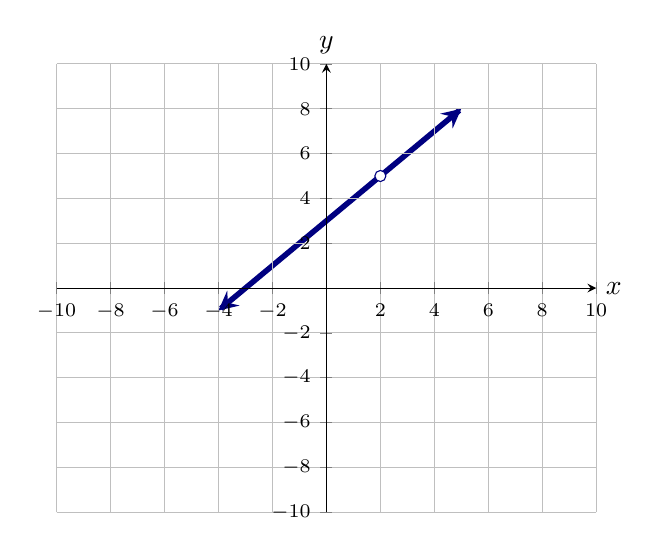
\begin{tikzpicture}
  \begin{axis}[
            domain=-10:10, ymax=10, xmax=10, ymin=-10, xmin=-10,
            axis lines =center, xlabel={$x$}, ylabel={$y$}, grid = major,
            ytick={-10,-8,-6,-4,-2,2,4,6,8,10},
            xtick={-10,-8,-6,-4,-2,2,4,6,8,10},
            ticklabel style={font=\scriptsize},
            every axis y label/.style={at=(current axis.above origin),anchor=south},
            every axis x label/.style={at=(current axis.right of origin),anchor=west},
            axis on top
          ]
          
            \addplot [line width=2, penColor, smooth,samples=100,domain=(-4:5),<->] {x+3};

          \addplot[color=penColor,fill=white,only marks,mark=*] coordinates{(2,5)};
          %\addplot[color=penColor,fill=penColor,only marks,mark=*] coordinates{(2,-2)};


  \end{axis}
\end{tikzpicture}
\end{image}
Here, $h(2)$ does not exist.   However, the pattern ``around'' $2$ suggests that $h(2)$ ``should'' be $5$. That would have fit our pattern better.







Graph of $y = G(r)$.

\begin{image}
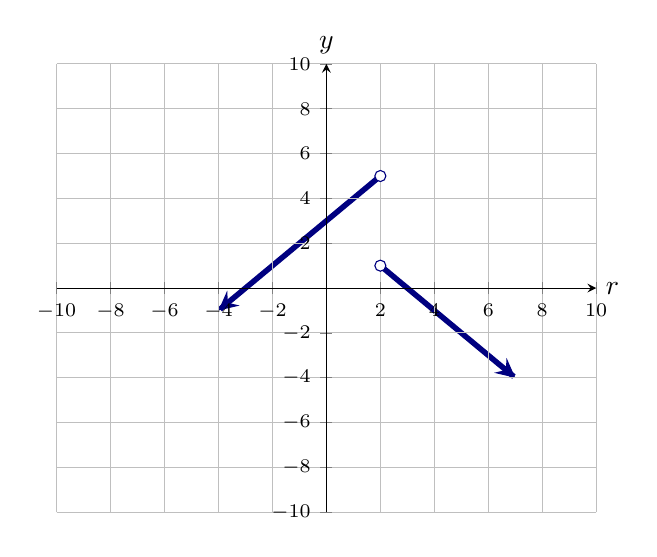
\begin{tikzpicture}
  \begin{axis}[
            domain=-10:10, ymax=10, xmax=10, ymin=-10, xmin=-10,
            axis lines =center, xlabel={$r$}, ylabel={$y$}, grid = major,
            ytick={-10,-8,-6,-4,-2,2,4,6,8,10},
            xtick={-10,-8,-6,-4,-2,2,4,6,8,10},
            ticklabel style={font=\scriptsize},
            every axis y label/.style={at=(current axis.above origin),anchor=south},
            every axis x label/.style={at=(current axis.right of origin),anchor=west},
            axis on top
          ]
          
            \addplot [line width=2, penColor, smooth,samples=100,domain=(-4:2),<-] {x+3};
            \addplot [line width=2, penColor, smooth,samples=100,domain=(2:7),->] {-x+3};

          \addplot[color=penColor,fill=white,only marks,mark=*] coordinates{(2,5)};
          \addplot[color=penColor,fill=white,only marks,mark=*] coordinates{(2,1)};


  \end{axis}
\end{tikzpicture}
\end{image}



We now have two expectations for the same domain number. The left side of our brain is expecting $G(2)=5$ and the right side of our brain is expecting $G(2)=1$. Both of these expectations come up empty, because $G$ has no value at $2$. \\







Graph of $y = r(t)$.  

\begin{image}
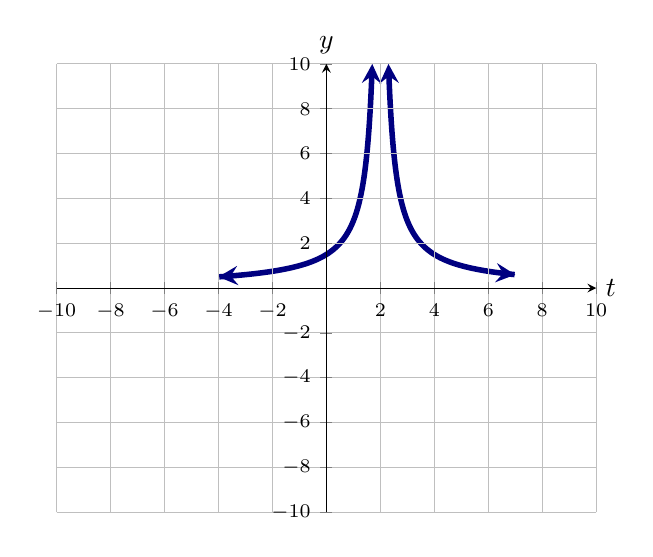
\begin{tikzpicture}
  \begin{axis}[
            domain=-10:10, ymax=10, xmax=10, ymin=-10, xmin=-10,
            axis lines =center, xlabel={$t$}, ylabel={$y$}, grid = major,
            ytick={-10,-8,-6,-4,-2,2,4,6,8,10},
            xtick={-10,-8,-6,-4,-2,2,4,6,8,10},
            ticklabel style={font=\scriptsize},
            every axis y label/.style={at=(current axis.above origin),anchor=south},
            every axis x label/.style={at=(current axis.right of origin),anchor=west},
            axis on top
          ]
          
            \addplot [line width=2, penColor, smooth,samples=200,domain=(-4:1.7),<->] {3/(2-x)};
            \addplot [line width=2, penColor, smooth,samples=200,domain=(2.3:7),<->] {3/(x-2)};

          %\addplot[color=penColor,fill=penColor,only marks,mark=*] coordinates{(2,1)};
        


  \end{axis}
\end{tikzpicture}
\end{image}



This one feels a little better, because we are expecting unboundedness.  But, there is still a single domain number that suddenly has no value, when all of the surrounding domain values have associated function values.












These examples illustrate that our internal intuition for function behavior is not always met.  But, that, in and of itself, is interesting.  Perhaps we can describe our expectations and compare those to the actual function.







Of course, not every open dot on the graph contradicts our expectations. Or, posseses any surprise at all.






Graph of $y = p(w)$.

\begin{image}
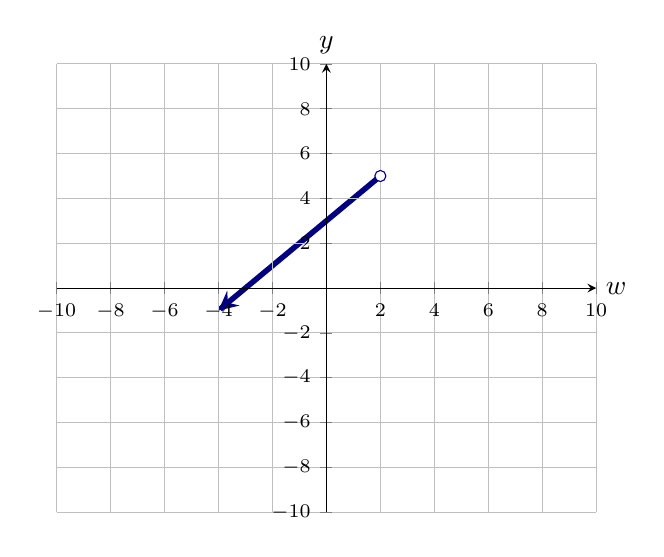
\begin{tikzpicture}
  \begin{axis}[
            domain=-10:10, ymax=10, xmax=10, ymin=-10, xmin=-10,
            axis lines =center, xlabel={$w$}, ylabel={$y$}, grid = major,
            ytick={-10,-8,-6,-4,-2,2,4,6,8,10},
            xtick={-10,-8,-6,-4,-2,2,4,6,8,10},
            ticklabel style={font=\scriptsize},
            every axis y label/.style={at=(current axis.above origin),anchor=south},
            every axis x label/.style={at=(current axis.right of origin),anchor=west},
            axis on top
          ]
          
            \addplot [line width=2, penColor, smooth,samples=100,domain=(-4:2),<-] {x+3};

          \addplot[color=penColor,fill=white,only marks,mark=*] coordinates{(2,5)};
          %\addplot[color=penColor,fill=penColor,only marks,mark=*] coordinates{(2,-3)};


  \end{axis}
\end{tikzpicture}
\end{image}








In the first three examples, right in the middle of the domain interval, the function suddenly vanishes away from its nice pattern. 

In this example, the domain is again a single interval, but the domain interval itself stops. The domain interval doesn’t include the endpoint, which makes it natural for the graph not to include the endpoint and for the function not to have a point there.

Since the domain interval itself doesn't include the endpoint, it is not bothersome that there is no function value there.








 
Graph of $y = G(x)$.
 
\begin{image}
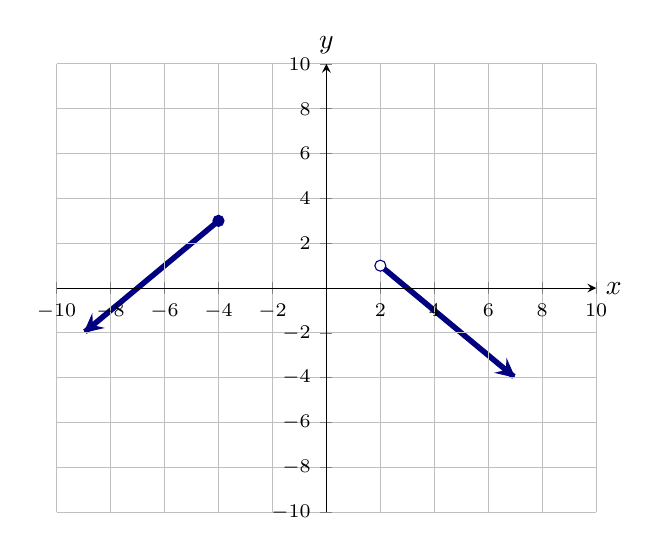
\begin{tikzpicture}
  \begin{axis}[
            domain=-10:10, ymax=10, xmax=10, ymin=-10, xmin=-10,
            axis lines =center, xlabel={$x$}, ylabel={$y$}, grid = major,
            ytick={-10,-8,-6,-4,-2,2,4,6,8,10},
            xtick={-10,-8,-6,-4,-2,2,4,6,8,10},
            ticklabel style={font=\scriptsize},
            every axis y label/.style={at=(current axis.above origin),anchor=south},
            every axis x label/.style={at=(current axis.right of origin),anchor=west},
            axis on top
          ]
           
            \addplot [line width=2, penColor, smooth,samples=100,domain=(-9:-4),<-] {x+7};
            \addplot [line width=2, penColor, smooth,samples=100,domain=(2:7),->] {-x+3};
 
            \addplot[color=penColor,fill=penColor,only marks,mark=*] coordinates{(-4,3)};
            \addplot[color=penColor,fill=white,only marks,mark=*] coordinates{(2,1)};
 
 
  \end{axis}
\end{tikzpicture}
\end{image}
 
 
 
 
 
In this example, the domain consists of two intervals, with space between them. One endpoint is include and the other is not.  The space makes all the difference.  \\



We base many of our expectations on space.  Where is there empty space?  Where is space filled in? \\

































\begin{idea}  \textbf{\textcolor{purple!85!blue}{What's catching our eye?}}


Our expectations from the patterns we see are disrupted when close domain numbers don't have close function values.


\end{idea}

This time there isn't a different value than we expected.  Instead, there is no value where we expected one. How do we compare function values to no function value? \\

We don't.

Again, we compare function values to themselves. \\


\begin{quote}
 \textbf{\textcolor{blue!55!black}{For domain numbers really really really close to $2$, the function values of $K$ for those domain numbers are not ALWAYS close to each other.}} 
\end{quote}


\begin{quote}
 \textbf{\textcolor{blue!55!black}{For domain numbers really really really close to $2$, the function values of $K$ for those domain numbers are close to each other, however, there is a missing value.}} 
\end{quote}




\textbf{\textcolor{red!70!darkgray}{$\blacktriangleright$}} We need a way of algebracially representing ``really close''.  \\


We also want to indicate the type of expectation we experienced that was interrupted with a missing domain number. So, we need to talk about domain numbers ``around'' the single domain number under observation. 


\textbf{\textcolor{red!70!darkgray}{$\blacktriangleright$}} We need to ensure that there is some filled in space ``around'' our domain number. \\





Another issue lurking in the shadows is that we always have the goal of \textbf{\textcolor{red!70!black}{all}}. Whenever we get ready to say something about this type of function behvior, we want our statement to apply to \textbf{\textcolor{red!70!black}{all}} of these situations. \\

We need to make sure that we avoid the most extreme and ridiculous situations.  We need to make sure that there is \textbf{\textcolor{red!70!black}{ALWAYS}} filled in space around our domain number.




\textbf{\textcolor{red!70!darkgray}{$\blacktriangleright$}} Open intervals are the tool of choice here.














\begin{center}
\textbf{\textcolor{green!50!black}{ooooo-=-=-=-ooOoo-=-=-=-ooooo}} \\

more examples can be found by following this link\\ \link[More Examples of Broken Values]{https://ximera.osu.edu/csccmathematics/precalculus/precalculus/functionValues/examples/exampleList}

\end{center}









\end{document}
